% =====================================================================
% Paper JSAC
% Body digital twin in the multi-user mmWave precoder loop:
% closed-form exposure-constrained precoding, scene path dictionary,
% and a plaza-scale operating regime
% Author: Robin Wydaeghe
% Target: IEEE JSAC Special Issue on Digital Twins for Wireless Networks
% =====================================================================

\documentclass[journal,twocolumn,10pt]{IEEEtran}

\usepackage[utf8]{inputenc}
\usepackage[T1]{fontenc}
\usepackage{lmodern}
\usepackage{microtype}

\usepackage{amsmath,amssymb,amsthm,mathtools}
\usepackage{bm}

\usepackage{graphicx}
\graphicspath{{figures/}{figures/jsac/}{../../theory/figures/}{../../validation/}{../../JSAC/code/experiments/rank_check/}{../../JSAC/code/experiments/cauchy_tightness/}{../../JSAC/code/experiments/csi_calibration/}{../../JSAC/code/experiments/tier_c_decision/}{../../JSAC/code/experiments/plaza_run/figures/}}
\usepackage{booktabs}
\usepackage{array}
\usepackage{caption}
\usepackage{subcaption}

\usepackage{cite}
\usepackage{xcolor}
\usepackage[colorlinks=true,linkcolor=blue,citecolor=blue,urlcolor=blue]{hyperref}
\usepackage[capitalize,nameinlink]{cleveref}

\theoremstyle{plain}
\newtheorem{theorem}{Theorem}
\newtheorem{proposition}[theorem]{Proposition}
\newtheorem{corollary}[theorem]{Corollary}
\theoremstyle{remark}
\newtheorem{remark}[theorem]{Remark}

\crefname{proposition}{Proposition}{Propositions}
\Crefname{proposition}{Proposition}{Propositions}
\crefname{corollary}{Corollary}{Corollaries}
\Crefname{corollary}{Corollary}{Corollaries}
\crefname{remark}{Remark}{Remarks}
\Crefname{remark}{Remark}{Remarks}
\crefname{theorem}{Theorem}{Theorems}
\Crefname{theorem}{Theorem}{Theorems}

\newcommand{\khat}{\hat{\bm{k}}}
\newcommand{\nhat}{\hat{\bm{n}}}
\newcommand{\rr}{\mathbf{r}}
\newcommand{\xx}{\mathbf{x}}
\newcommand{\hh}{\mathbf{h}}
\newcommand{\ww}{\mathbf{w}}
\newcommand{\gvec}{\mathbf{g}}
\newcommand{\bvec}{\mathbf{b}}
\newcommand{\Sinc}{S_{\mathrm{inc}}}
\newcommand{\Sab}{S_{\mathrm{ab}}}
\newcommand{\Pabs}{P_{\mathrm{abs}}}
\newcommand{\Aab}{A_{\mathrm{ab}}}
\newcommand{\Aperp}{A_\perp}
\newcommand{\GG}{\mathbf{G}}
\newcommand{\Gtil}{\tilde{\mathbf{G}}}
\newcommand{\Qmat}{\mathbf{Q}}
\newcommand{\Mmat}{\mathbf{M}}
\newcommand{\Jmat}{\mathbf{J}}
\newcommand{\Pmat}{\mathbf{P}}
\newcommand{\Phimat}{\mathbf{\Phi}}
\newcommand{\Psimat}{\bm{\Psi}}
\newcommand{\Psitil}{\tilde{\bm{\Psi}}}
\newcommand{\Fn}{\mathbf{F}_n}
\newcommand{\psin}{\bm{\psi}_n}
\newcommand{\diff}{\mathrm{d}}
\newcommand{\Complex}{\mathbb{C}}
\newcommand{\ntilde}{\tilde{n}}
\newcommand{\AllBodies}{\mathcal{P}}
\newcommand{\Served}{\mathcal{U}}
\newcommand{\Bystanders}{\mathcal{B}}
\newcommand{\Dict}{\mathcal{D}}
\DeclareMathOperator{\ReLU}{ReLU}
\DeclareMathOperator{\RE}{Re}
\DeclareMathOperator{\IM}{Im}
\DeclareMathOperator{\tr}{tr}

\title{Body digital twin in the multi-user
millimetre-wave precoder loop}

\author{Robin~Wydaeghe%
  \thanks{R. Wydaeghe is with Ghent University and imec, Ghent, Belgium
  (e-mail: robin.wydaeghe@ugent.be).}}

\markboth{IEEE Journal on Selected Areas in Communications,
  Vol.~XX, No.~X, Month~2026}%
{Wydaeghe: Body digital twin in the multi-user mmWave precoder loop}

\begin{document}

\maketitle

\begin{abstract}
Reference-level electromagnetic-field caps in several European
jurisdictions, including the Brussels capital region's $14.57\,$V/m
cumulative outdoor limit and the Italian attention values, restrict
millimetre-wave downlink deployment more tightly than propagation
physics does. We treat each body in the cell as an instance of a
digital twin maintained inside the base-station control loop and
close that loop against per-body absorbed-power budgets. The twin
couples three ingredients. A coherent exposure operator
$\Qmat^{(u)} \in \Complex^{M \times M}$ on the precoder, computed
from ray-traced propagation paths, returns whole-body absorbed power
as a Hermitian quadratic form. A scene path dictionary is built once
by ray tracing over the static base-station-and-scene geometry,
indexed by body position, and calibrated at runtime against served-user
uplink CSI. A tiered telemetry mapping turns served users, cooperating
non-users, and sensed bystanders into twin instantiations of
decreasing position-and-pose fidelity. Multi-user sum-rate maximisation
under per-body exposure caps admits the closed-form precoder
$\ww_k^\star = (\Qmat_{\mathrm{tot}}(\bm\lambda) + \nu\,\mathbf{I})^{-1}
\gvec_k$, in which the rank-one degenerate limit recovers regularised
zero-forcing. The loop runs on the Brussels Grand Place geometry with
50 SMPL-X bodies on AMASS walk-cycles, an $8 \times 8$ panel at
$26\,$GHz, and 25 served users. The empirical exposure operator has
effective rank 3 to 4 at the $99\,\%$ trace fraction in both a
plaza-specular path model and the 3GPP UMa-LOS stochastic model.
GPU $\Qmat$-refresh is $7.5\,$ms per body and the closed-form
multi-body precoder solves at $31\,$ms median for $K = B = 25$ and
$M = 64$. The Brussels reference-level budget is satisfied at every
body-slot in the canonical plaza load by about four orders of
magnitude, and the five precoders we compare (MRT, ZF, worst-case
back-off, the proposed multi-body ECBF, and a pose-known oracle)
collapse to one operating point under that slack. Chronic-dose
ECDFs stratified by tier give the practical value: cooperating
non-users absorb $0.40\times$ of the served-user median over a
$20\,$s walk-cycle window, bystanders absorb $0.92\times$. The
conditional bound on $\xx^H \Qmat^{(u)} \xx$ that follows from the
projected-area Cauchy formula is loose by 21 to $27\,$dB on the
line-of-sight steering direction and is breached by 49 to $70\,\%$
of random and ECBF precoders, tracing to the geometric mismatch
between the leading exposure mode and the BS-side steering vector.
\end{abstract}

\begin{IEEEkeywords}
Digital twin, exposure-constrained beamforming, MIMO, millimetre wave,
ICNIRP compliance, ray tracing, multi-user precoding,
electromagnetic-field reference level.
\end{IEEEkeywords}

\IEEEpeerreviewmaketitle


\section{Introduction}\label{sec:intro}
\IEEEPARstart{F}{ifth-generation} and emerging sixth-generation
networks deploy multi-element antenna arrays at millimetre-wave
frequencies and operate them at short range from human users. The
2020 ICNIRP guidelines~\cite{ICNIRP2020} replace whole-body specific
absorption rate above 6\,GHz with absorbed power density on the body
surface and tighten local limits at the same distances where mobile
and fixed-wireless devices operate. Several European jurisdictions
enforce stricter local reference levels: the Brussels capital region
caps the cumulative outdoor field at $14.57\,$V/m, equivalent to
$0.56\,$W/m$^2$ time-averaged in the radiating
band~\cite{BrusselsArrete2007,BrusselsArrete2024}, and Italy maintains
attention values at $6$ to $15\,$V/m depending on
exposure category~\cite{ItalyDL}. These caps are conservative
free-space proxies for the tissue-protection basic restrictions from
which they descend. ICNIRP allows compliance to be shown via
direct evaluation of the basic restriction~\cite{IEC62232}, but no
deployed mechanism yet performs that evaluation in real time on a
moving population. The deployment blocker is therefore not propagation
physics but a per-body, per-slot dosimetry that the network does not
currently maintain.

The standard tool for exposure-aware beamforming is the SAR-matrix
formulation of Hochwald et al.~\cite{Hochwald2014}. Whole-body
absorbed power for an $M$-element array is a Hermitian quadratic form
$\xx^H \mathbf{S} \xx$ in the precoder. Ying et
al.~\cite{Ying2015} solved the exposure-constrained signal-to-noise
problem and derived the closed-form precoder
$\xx^\star \propto (\lambda \mathbf{S} + \nu \mathbf{I})^{-1} \hh^*$.
Variants extend to multi-user
MIMO~\cite{Ying2017} and to robust precoding under channel
uncertainty. In every published instance, $\mathbf{S}$ is calibrated
numerically by full-wave finite-difference time-domain simulation per
device per body configuration. The construction is single-body and
single-pose, and the calibration assumes a fixed array-body geometry
known offline. Castellanos and Heath~\cite{Castellanos2020} reduce the
calibration cost at 28\,GHz by replacing the matrix with per-element
scalar Fresnel coefficients on a sphere model. Concurrent work on
SAR-aware parallel-transmit MRI~\cite{MeliadoSAR2020,GokyarpTx2023} and
on uplink exposure-aware beamforming under thermal
constraints~\cite{ZhouUL2026} shares the matrix machinery but operates
on fixed birdcage geometries or single handsets. None of these
formulations represent more than one body, none use a runtime,
network-side ray tracer, and none close a loop over a moving
population.

A body-side digital twin is the natural object that ties the matrix
machinery to a moving population. Each body in the coverage cell
carries an exposure operator $\Qmat^{(u)} \in \Complex^{M \times M}$
that depends on the body's geometry, pose, and position. The base
station maintains a per-body twin and applies a precoder that
satisfies a budget on $\xx^H \Qmat^{(u)} \xx$ for every $u$. The
question this paper answers is what such a twin actually needs from
the body, what it can recover from the network's own ray-traced
channel state, and how the closed loop behaves in a realistic plaza
scenario.

The contribution is a closed-loop, multi-body, body-side digital twin
together with an empirical characterisation of its operating regime.
Three components do the work. A coherent exposure operator $\Qmat^{(u)}$
is computed from per-path Fresnel transmission on a per-body mesh
under two cross-term approximations bounded at $\leq 5\,\%$ on
$\xx^H \Qmat^{(u)} \xx$ for any precoder. A scene path dictionary is
built once by ray tracing over the static base-station-and-scene
geometry, indexed by body position, and calibrated at runtime by
least-squares regression of path amplitudes against served-user
uplink CSI. Multi-user sum-rate maximisation under $K + B$ per-body
exposure caps admits the closed-form precoder
$\ww_k^\star = (\Qmat_{\mathrm{tot}}(\bm\lambda) + \nu \mathbf{I})^{-1}
\gvec_k$ with KKT bisection on the dual variables, a generalisation of
Ying-2015 to a heterogeneous body population that retains the
closed-form structure and reduces to regularised zero-forcing in the
rank-one degenerate limit. The empirical contribution is a
plaza-scale evaluation of the loop on the Brussels Grand Place
geometry with 50 SMPL-X bodies on AMASS walk-cycles and an
$8 \times 8$ panel at 26\,GHz: the operator has effective rank 3 to 4,
GPU $\Qmat$-refresh fits within $100\,$ms per pose update, and the
multi-body precoder solves at $31\,$ms median. The Brussels reference
level is slack by about four orders of magnitude at this load, so the
five precoders we compare collapse to one operating point. Chronic-dose
ECDFs separate by tier and give the practical value proposition. The
projected-area-based bound on $\xx^H \Qmat^{(u)} \xx$ that does not
condition on the steering direction is loose by 21 to 27\,dB on a
line-of-sight worst-case precoder and is breached by random and ECBF
precoders, which we trace to the geometric mismatch between the
leading exposure mode and the BS steering vector.

The remainder of the paper is organised as follows.
\Cref{sec:setup} fixes notation and assembles the per-body exposure
operator from a common ray-traced path set, with a two-line summary
of the closed-form derivation needed downstream. \Cref{sec:precoder}
formulates the multi-user sum-rate problem under per-body exposure
caps and derives the closed-form solver and its zero-forcing limit.
\Cref{sec:twin} describes the scene path dictionary, the runtime CSI
calibration, the tiered telemetry mapping, and the closed-loop
cadence. \Cref{sec:eval} reports the Brussels Grand Place evaluation,
including the rank, runtime, hero, chronic-dose, ablation, ISAC
detection, and calibration figures. \Cref{sec:regulatory} lays out
the basic-restriction audit pathway and the reference-level footprint
argument. \Cref{sec:discussion} discusses what the operating regime
implies for deployment, where the bound conditions matter, and the
limitations of the present evaluation. \Cref{sec:conclusion} closes.


\section{System model and per-body exposure operator}\label{sec:setup}

A base station has $M$ antenna elements and radiates with precoder
$\xx \in \Complex^M$ such that $\|\xx\|^2 \leq P_{\mathrm{tx}}$. The
propagation environment between the array and any point in the cell
produces $N$ paths via reflection, scattering, and diffraction. Path
$n$, for $n = 1, \ldots, N$, has originating array element
$j(n) \in \{1, \ldots, M\}$, arrival direction $\khat_n$ at the body
surface, and complex polarisation-amplitude vector
$\psin \in \Complex^3$ orthogonal to $\khat_n$ that encodes the
amplitude, polarisation state, and propagation phase along the path.
The base station's ray tracer computes
$\{j(n), \khat_n, \psin\}_{n=1}^N$ for any spatial probe point,
including each user-equipment position $\rr_{\mathrm{UE}}$ and each
body location.

The path-space machinery uses three matrices. The element-to-path
dispatch is $\Jmat \in \{0, 1\}^{N \times M}$, with
$J_{nj} = \delta_{j(n), j}$. For an observation point
$\rr \in \mathbb{R}^3$, the phase diagonal is
$\Phimat(\rr) = \mathrm{diag}(e^{-i k_0 \khat_1 \cdot \rr}, \ldots,
e^{-i k_0 \khat_N \cdot \rr})$. The polarisation matrix stacks the
per-path polarisation-amplitude vectors as columns,
$\Psimat = [\bm\psi_1, \ldots, \bm\psi_N] \in \Complex^{3 \times N}$.
The free-space electric field at any point $\rr$ under precoder $\xx$
is
\begin{equation}\label{eq:E-decomp}
  \mathbf{E}(\rr) = \GG(\rr)\,\xx,
  \qquad
  \GG(\rr) = \Psimat\,\Phimat(\rr)\,\Jmat \in \Complex^{3 \times M}.
\end{equation}
The user-equipment received signal at $\rr_{\mathrm{UE}}$ is
$y(\xx) = \hh^T \xx$, with $\hh^* = \Jmat^T \bvec$ and
$\bvec = \Phimat(\rr_{\mathrm{UE}})^H \bm\alpha^*$ collecting the
per-path antenna projections
$\alpha_n = \mathbf{C}_R(\khat_n)^H \psin$. The channel is the
ordinary 3GPP NR channel, written in path space.

\subsection{Per-body coherent absorption law}\label{sec:cohlaw}

At a body-surface point $\rr$ with outward normal $\nhat(\rr)$, path
$n$ has incidence cosine $\mu_n = \nhat(\rr)\cdot(-\khat_n)$. For a
front-facing path ($\mu_n > 0$), the incident plane-wave field
refracts and decays inside the tissue half-space with depth-coupling
exponent $k_0 \xi_n = \beta_n - i \alpha_n^{(d)}$, with
$\xi_n = \sqrt{\ntilde^2 - 1 + \mu_n^2}$. Two cross-term
approximations collapse the coherent depth integral to a squared
norm. The first replaces the refracted TM polarisation direction
inside tissue by the incident TM direction, with cross-term error
$O(1/|\ntilde|^2) \leq 4\,\%$ at 26\,GHz on skin. The second sets the
normalised depth coupling between path pairs to unity, with maximum
cross-term error $0.44\,\%$ over $[0^\circ, 85^\circ]^2$. Self-terms
are exact under both approximations. Define the tissue-weighted
per-path read-out
\begin{equation}\label{eq:psitil}
  \tilde{\bm\psi}_n(\rr) = \sqrt{\frac{\sigma}{4\,\alpha_n^{(d)}}}\,
  \Fn(\rr)\,\psin \in \Complex^3,
\end{equation}
where $\Fn(\rr)$ is the per-path Fresnel transmission operator that
maps the incident polarisation amplitude to its TE-and-TM-filtered
version on the surface. Stack
$\Psitil(\rr) = [\tilde{\bm\psi}_1(\rr), \ldots,
\tilde{\bm\psi}_N(\rr)] \in \Complex^{3 \times N}$. The body-surface
field channel is
\begin{equation}\label{eq:Gtilde}
  \Gtil(\rr) = \Psitil(\rr)\,\Phimat(\rr)\,\Jmat
  \in \Complex^{3 \times M},
\end{equation}
with the same $(\Phimat, \Jmat)$ structure as the free-space field.
The absorbed power density at $\rr$ is then
$\Sab(\rr) = \|\Gtil(\rr)\,\xx\|^2$. The combined cross-term error on
$\Sab$ is bounded at $\leq 5\,\%$ for any precoder. \Cref{app:fresnel}
collects the explicit form of $\Fn(\rr)$.

\subsection{Per-body exposure operator}\label{sec:Q}

Integrating the absorption law over the surface of body $u$ gives a
Hermitian quadratic form in the precoder. The per-body exposure
operator is
\begin{equation}\label{eq:Q-def}
  \Qmat^{(u)} = \int_{\Sigma^{(u)}} \Gtil(\rr)^H\,\Gtil(\rr)\,\diff A
  \in \Complex^{M \times M},
\end{equation}
so that $\Pabs^{(u)}(\xx) = \xx^H \Qmat^{(u)} \xx$ is the whole-body
absorbed power on body $u$ under precoder $\xx$. $\Qmat^{(u)}$ is
Hermitian positive-semidefinite by construction, with rank at most
$\min(M, 3 M_\Sigma)$ where $M_\Sigma$ is the number of integration
triangles on the body mesh. The eigendecomposition
$\Qmat^{(u)} = \sum_k \lambda_k \mathbf{v}_k \mathbf{v}_k^H$ with
$\lambda_1 \geq \cdots \geq \lambda_M \geq 0$ are the body's exposure
modes. The trace $\tr(\Qmat^{(u)})$ equals the expected absorbed
power on body $u$ under isotropic random precoding, scaled by
transmit power.

The path-space structure of $\Qmat^{(u)}$ separates the array
hardware from the body and the scene. From
$\Gtil(\rr) = \Psitil(\rr) \Phimat(\rr) \Jmat$,
\begin{equation}\label{eq:Q-factor}
  \Qmat^{(u)} = \Jmat^T\,\Mmat^{(u)}\,\Jmat,
  \qquad
  \Mmat^{(u)} = \int_{\Sigma^{(u)}} \Phimat^H \Psitil^H \Psitil\,
  \Phimat\,\diff A,
\end{equation}
where $\Mmat^{(u)} \in \Complex^{N \times N}$ is the per-body path-pair
Gram. The dispatch $\Jmat$ is combinatorial and depends only on the
array hardware and the ray tracer's path counting. The Gram
$\Mmat^{(u)}$ depends only on the body geometry, body pose, and the
arrival path set at the body's location. The position dependence of
$\Qmat^{(u)}$ enters through a translation phasor identity that we
return to in \cref{sec:twin}.

\subsection{Multi-body aggregation}\label{sec:aggregation}

For a population $\AllBodies = \Served \cup \Bystanders$ of $|\Served|
= K$ served users and $|\Bystanders| = B$ bystanders, the base station
maintains $K + B$ operators $\{\Qmat^{(u)}\}_{u \in \AllBodies}$ and
radiates $\xx_{\mathrm{total}} = \sum_{k=1}^K \ww_k s_k$ with
zero-mean unit-variance mutually uncorrelated symbols $s_k$. Taking
expectations over the symbol set, the time-averaged absorbed power
on body $u$ decomposes across served streams:
\begin{equation}\label{eq:Pabs-MU}
  \Pabs^{(u)} = \sum_{k=1}^K \ww_k^H\,\Qmat^{(u)}\,\ww_k.
\end{equation}
Both served users and bystanders contribute exposure constraints. The
geometry of the path set on body $u$, not the body's role as a
served user, determines how heavily $u$ couples to a candidate
precoder.


\section{Multi-user precoder under per-body exposure caps}\label{sec:precoder}

The multi-user sum-rate maximisation problem with $K + B$ per-body
exposure budgets is the QCQP
\begin{equation}\label{eq:P-MB}
\begin{aligned}
  \max_{\{\ww_k\}_{k=1}^K} \;& R_{\mathrm{sum}}(\{\ww_k\}) \\
  \text{s.t.}\;& \Pabs^{(u)} \leq L^{(u)},\quad u \in \AllBodies,\\
  & \sum_{k=1}^K \|\ww_k\|^2 \leq P_{\mathrm{tx}},
\end{aligned}
\end{equation}
where $R_{\mathrm{sum}}$ is the achievable sum-rate and $L^{(u)}$ is
the absorbed-power budget on body $u$, set by the binding regulatory
regime. The feasible set is the intersection of $K + B$ PSD ellipsoids
in $\bigoplus_k \Complex^M$ with the $\ell_2$ ball.

\subsection{Closed-form solver}

The weighted-MMSE surrogate of Christensen et
al.~\cite{Christensen2008} and Shi et al.~\cite{Shi2011} replaces the
sum-rate by an iteratively reweighted quadratic objective. Aggregating
the exposure dual variables into $\bm\lambda \in \mathbb{R}_+^{K+B}$
and the power dual into $\nu \geq 0$, the KKT stationarity condition
of the inner reweighted problem fixes $\ww_k$ in closed form. Define
the aggregate exposure operator
\begin{equation}\label{eq:Qtot}
  \Qmat_{\mathrm{tot}}(\bm\lambda) =
  \sum_{u \in \AllBodies} \lambda_u\,\Qmat^{(u)},
\end{equation}
also Hermitian positive-semidefinite. Define the per-stream
weighted-MMSE drive vector $\gvec_k$ as the canonical
weighted-MMSE pseudo-channel whose precise form follows
Shi-2011~\cite{Shi2011} and is reproduced in \cref{app:ecbf}. The
inner stationarity gives
\begin{equation}\label{eq:closedform}
  \boxed{\;
  \ww_k^\star =
  \bigl(\Qmat_{\mathrm{tot}}(\bm\lambda) + \nu\,\mathbf{I}\bigr)^{-1}\,
  \gvec_k.\;}
\end{equation}
The dual variables $(\bm\lambda, \nu)$ are determined by
complementary slackness on the active exposure and power constraints.
\Cref{app:ecbf} writes out the dual ascent: the inner inverse is
solved at fixed $\bm\lambda$, the constraint residuals are evaluated,
and a Newton step on $\bm\lambda$ updates the active set. In our
implementation, dual ascent reaches machine-precision residuals in
10 to 30 outer iterations from a cold start, against 800 to
$1{,}600$ Gauss-Seidel sweeps for the same accuracy.

\begin{remark}[Specialisations]\label{rem:limits}
\Cref{eq:closedform} contains every standard mmWave precoder as a
special case. With $\bm\lambda = 0$, the matrix
$\Qmat_{\mathrm{tot}}$ vanishes and $\ww_k^\star \propto \gvec_k$
reduces, after the WMMSE outer fixed point, to MRT for $K = 1$ or to
regularised channel-inversion zero-forcing for $K > 1$. With
$\bm\lambda \to \infty$ on tight constraints, the precoder steers
into the joint absorption null space.
\end{remark}

\subsection{Zero-forcing as a rank-one degenerate limit}

The classical zero-forcing precoder is the rank-one limit of
\cref{eq:closedform}.

\begin{proposition}[ZF as the rank-one limit]\label{prop:ZFlimit}
Suppose every per-body exposure operator degenerates to a rank-one
form $\Qmat^{(u)} = \sigma_u\,\mathbf{a}_u\,\mathbf{a}_u^H$, with
$\mathbf{a}_u \in \Complex^M$ the body's BS-side equivalent steering
vector. Stack the steering vectors as the rows of $\mathbf{A}
\in \Complex^{(K+B)\times M}$, the dual-weighted diagonal as
$\mathbf{D} = \mathrm{diag}(\lambda_u \sigma_u)$, and the regularised
inverse as $(\mathbf{A}^H \mathbf{D} \mathbf{A} + \nu \mathbf{I})^{-1}$.
Then \cref{eq:closedform} reduces to the regularised zero-forcing
precoder of Peel-Hochwald-Swindlehurst~\cite{PeelHochwald2005}
applied to the heterogeneous user-and-bystander steering set.
\end{proposition}

The proof is direct substitution in \cref{eq:Qtot}. The rank-one
limit is informative: it shows that the multi-body exposure
constraint generalises zero-forcing rather than competing with it.
With each body collapsed to a scalar steering direction,
\cref{eq:closedform} matches the classical receiver-aware
regularised inversion. With $\Qmat^{(u)}$ retaining higher rank, the
solver smoothly degrades hard nulls into soft-budget back-offs that
spend less precoder DoF.

\subsection{Soft budgets and DoF cost}\label{sec:softbudget}

Hard nulls consume one precoder DoF per body and saturate at
$K + B \approx M$. Soft budgets $L^{(u)} > 0$ cost less: in the
plaza-scale evaluation of \cref{sec:eval}, $K + B = 50$ on $M = 64$,
which would already be near-singular under hard nulls but is well
within the closed-form regime under soft budgets. The empirical rank
of $\Qmat^{(u)}$ in the same scenario is 3 to 4 at the 99\,\% trace
fraction (\cref{sec:rank-eval}), so $\Qmat_{\mathrm{tot}}$ has at
most $\sim 4(K+B) = 200$ effective directions, again well above the
$M = 64$ array dimension. The closed-form solver inherits this
regime structurally.


\section{Body twin, scene path dictionary, and tiered
telemetry}\label{sec:twin}

The exposure operator $\Qmat^{(u)}$ depends on three classes of
quantity, each varying on its own timescale. The base station's
location and the static scene geometry change on infrastructure
timescales. The bodies' positions change at walking pace, on the
order of $1\,$s for a metre of displacement. The bodies' poses change
at $\sim 100\,$ms. Per-slot CSI for served users updates at the
$1\,$ms PHY frame. The twin design separates these timescales so
that each cadence carries only the work that genuinely changes at
that rate.

\subsection{Scene path dictionary}\label{sec:dict}

The static scene-and-array geometry produces a path set that depends
only on the location $\rr_0$ of the body's centre. Define the scene
path dictionary
\begin{equation}\label{eq:dict-def}
  \Dict = \bigl\{\bigl(\khat_n(\rr_0), \psin(\rr_0),
  \alpha_n^{(d)}(\rr_0), j(n)\bigr)\bigr\}_{\rr_0 \in \mathcal{G},\,n},
\end{equation}
where $\mathcal{G}$ is a discrete grid of plausible body centres in
the cell. For a $100 \times 100\,$m cell at a $1\,$m grid,
$|\mathcal{G}| = 10^4$. With at most 20 paths per probe point and
single-precision complex storage, $\Dict$ fits in tens of megabytes.
The dictionary is built once, offline, by running a differentiable ray
tracer~\cite{SionnaRT,DiffeRT} over the static scene with the panel
fixed. At runtime, the per-body Gram $\Mmat^{(u)}(\rr_0, \bm\theta_u)$
in body-local coordinates is the only quantity that varies with
pose. Translation to the body's actual position is then a diagonal
phasor:
\begin{equation}\label{eq:translation}
  \Mmat^{(u)}(\rr_0 + \mathbf{t}, \bm\theta_u) =
  \Phimat(\mathbf{t})^H\,\Mmat^{(u)}(\rr_0, \bm\theta_u)\,\Phimat(\mathbf{t}).
\end{equation}
\Cref{eq:translation} costs $O(N)$ complex exponentials and avoids
re-running the ray tracer on per-second body translations.

\subsection{Closing the in-silico to deployed-channel gap}\label{sec:csi-cal}

The dictionary's path directions are accurate to the geometric
resolution of the ray tracer. Path amplitudes are not. Real
deployments suffer from antenna calibration error, scatterer
material miscoincidence with the OSM database, and small-scale
feature loss in the OSM-and-3D-Tiles input. We close that gap by
fitting a complex per-path scale $\beta_n \in \Complex$ against
served-user uplink CSI. For each served user $k$, the twin computes
the in-silico channel $\hat\hh_k = \bm\alpha_k^T \Phimat(\rr_k)
\Jmat \in \Complex^M$ from the dictionary and obtains the measured
channel $\hh_k^{\mathrm{meas}}$ from uplink pilots. The amplitudes
solve the least-squares problem
\begin{equation}\label{eq:csi-LS}
  \hat{\bm\beta}_k = \arg\min_{\bm\beta \in \Complex^N}\;
  \bigl\|\hh_k^{\mathrm{meas}} - \mathrm{diag}(\bm\beta) \cdot
  \hat\hh_k\bigr\|^2 + \rho\,\|\bm\beta - \mathbf{1}\|^2,
\end{equation}
with ridge regularisation $\rho > 0$ that biases toward the
in-silico amplitudes. The fit propagates to every $\Qmat^{(u)}$
that shares dictionary entries with body $k$. \Cref{sec:eval-csi}
characterises the residual against perturbation amplitude and
operating SNR. The mechanism resembles channel-charting and
ray-trace-aided calibration~\cite{SionnaRT}, but the unknowns are
per-path complex scales over a known geometric set, not a learned
embedding.

\subsection{Tiered telemetry}\label{sec:tiers}

\Cref{tab:tiers} catalogues the practical mapping from a body's
operational state to the twin's instantiation. Served users (tier A)
report position from GPS and pose from on-phone IMU
filtering~\cite{Madgwick2011} streamed through the operator's
application channel. Cooperating non-users (tier B) carry an active
phone with uplink presence and no served traffic, and share the
same GPS and IMU stream. Non-cooperating bystanders (tier C) report
nothing, and the twin recovers their position from base-station-side
ISAC monostatic radar at the panel. We characterise the tier-C
detection regime in \cref{sec:eval-isac}. Bodies the twin cannot
detect (tier D) are handled by an occupancy envelope: a regulatory
construct that imposes a worst-case bystander on a coarse spatial
grid in sensing blind spots, treated as a fixed fallback that does
not bind under the canonical plaza load.

\begin{table}[!t]
\caption{Tiered body telemetry and twin instantiation.}
\label{tab:tiers}
\centering
\small
\begin{tabular}{@{}p{0.06\columnwidth}p{0.27\columnwidth}p{0.22\columnwidth}p{0.30\columnwidth}@{}}
\toprule
Tier & Body type & Position & Pose \\
\midrule
A & Served user & GPS, IMU & IMU--filtered SMPL pose \\
B & Cooperating non-user & GPS, IMU & IMU--filtered SMPL pose \\
C & Sensed bystander & BS--side ISAC RCS & Worst-case envelope \\
D & Undetected & Occupancy grid & Worst-case envelope \\
\bottomrule
\end{tabular}
\end{table}

\subsection{Refresh cadences and per-slot compute}\label{sec:cadence}

\Cref{tab:cadence} lists the refresh cadences and the empirical
per-update wall-clock time for each twin component. The CSI
calibration $\bm\beta_k$ runs at $\sim 1\,$s, gated by the LS
problem's overdetermination requirement (\cref{sec:eval-csi}). The
pose-driven $\Mmat^{(u)}$ refresh runs at $\sim 100\,$ms per body
and is the dominant per-body GPU cost. The translation phasor on
$\Mmat^{(u)}$ runs at $\sim 1\,$s per body, an $O(N)$ diagonal
update. The precoder solve runs at every PHY frame, with the
multi-body QCQP solver of \cref{sec:precoder} dispatching at
$31\,$ms median for $K = B = 25$ on $M = 64$. The cadence table
shows how the dual-decomposition naturally sits over the
two-timescale separation: slow operator updates feed a fast
precoder solver.

\begin{table}[!t]
\caption{Refresh cadence, per-update cost, and the source of cost.
RTX 3090, JAX backend, single-precision complex.}
\label{tab:cadence}
\centering
\small
\begin{tabular}{@{}p{0.32\columnwidth}p{0.13\columnwidth}p{0.42\columnwidth}@{}}
\toprule
Quantity & Cadence & Per-update time \\
\midrule
UE CSI $\hh_k$ & $1\,$ms & $O(M)$ from PHY pilots \\
Precoder $\ww_k^\star$ & $1\,$ms & $31\,$ms median solve, $K = B = 25$, $M = 64$ \\
Translation phasor $\Phimat(\mathbf{t}_u)$ & $\sim 1\,$s & $O(N)$ per body \\
Pose-driven $\Mmat^{(u)}$ & $\sim 100\,$ms & $7.5\,$ms per body, $\sim 2.4$\,k tri \\
Path dictionary $\Dict$ & static & offline ray tracer, minutes \\
CSI calibration $\bm\beta_k$ & $\sim 1\,$s & LS fit, $O(N M)$ \\
\bottomrule
\end{tabular}
\end{table}

The tabulated $1\,$ms precoder cadence is the slot rate, not the
solve time. The multi-body QCQP solve at $31\,$ms is amortised
across the slot, and warm-started across slots in production.


\section{Plaza-scale demonstration}\label{sec:eval}

The closed loop runs on a Brussels Grand Place geometry at $26\,$GHz
with an $8 \times 8 = 64$-element uniform rectangular array on a
facade at $8\,$m height with $10^\circ$ downtilt and $30\,$dBm
transmit power. The cell hosts 50 SMPL-X bodies on AMASS walk-cycle
traces~\cite{SMPL,SMPLX,AMASS} retargeted at $30\,$Hz: 25 served
users in tier A, 15 cooperating non-users in tier B, and 10 sensed
bystanders in tier C. Skin tissue at 26\,GHz takes
$\varepsilon_r = 16.55$, $\sigma = 25.8\,$S/m,
$\ntilde = 4.47 - 1.85i$ from the IT'IS database (v5.0). The path
dictionary is exercised in two regimes. A plaza-specular set
contains line-of-sight, ground reflection, and two facade reflections
per probe point. A stochastic 3GPP UMa-LOS set has 60 subpaths per
cluster~\cite{TR38901}. Per-body absorbed-power budgets are taken
from the Brussels reference level of $14.57\,$V/m
($S_{\mathrm{lim}} = 0.56\,$W/m$^2$), giving
$L^{(u)}_{\mathrm{RL}} \approx T_0 S_{\mathrm{lim}}
\Aab^{(u)}\bar\eta^{(u)} \approx 0.19\,$W per body for an adult of
$\Aab \approx 1.45\,$m$^2$ at $\bar\eta = 0.5$. The PHY surrogate is
Shannon capacity over the per-stream effective channel. We discuss
the Sionna NR PHY pass in \cref{sec:discussion}. The window is $20\,$s
of wall-clock-equivalent simulation, $600$ slots at $33\,$ms slot
spacing.

\subsection{When the cap binds}\label{sec:eval-binding}

The Brussels reference level binds inside a small range. Under
isotropic radiation at $30\,$dBm split across $K$ served users, the
incident power density at range $r$ is $S(r, K) = P_{\mathrm{tx}}/(4
\pi r^2 K)$. Equating $S(r, K)$ to one-quarter of $S_{\mathrm{lim}}$
(the residual budget for one operator under a four-operator
cumulative cap) gives binding distance
$r^\star(K) = (P_{\mathrm{tx}}/(\pi S_{\mathrm{lim}} K))^{1/2}$.
\Cref{tab:bind} tabulates $r^\star$ versus $K$. The plaza scenario
sits at $K = 25$ with bodies at $5$ to $55\,$m, well outside the
binding range. Under directional MRT the equivalent isotropic
radiated power is $K \cdot M = 64$ times larger per stream, but the
beam concentrates on the served user, so the bystander integration
is dominated by the side lobes, and the back-of-envelope places the
worst-case bystander at $r^\star_{\mathrm{MRT}}(K=25)
\sim 4$ to $6\,$m, still inside the geometric exclusion of the
panel. The closed-loop machinery therefore does most of its work in
the slack regime, with chronic dose as the binding metric for
sustained operation.

\begin{table}[!t]
\caption{Brussels reference-level binding distance $r^\star(K)$ for
isotropic equal-power split, $30\,$dBm transmit, four-operator
cumulative cap. Beyond $r^\star$, the cap is slack.}
\label{tab:bind}
\centering
\small
\begin{tabular}{@{}c c@{}}
\toprule
Served users $K$ & Binding distance $r^\star$ \\
\midrule
1 & $13.4\,$m \\
5 & $6.0\,$m \\
10 & $4.2\,$m \\
25 & $2.7\,$m \\
\bottomrule
\end{tabular}
\end{table}

\subsection{Empirical operator structure}\label{sec:rank-eval}

\Cref{fig:rank-cdf} shows the empirical rank of $\Qmat^{(u)}$ over
20 Thelonious bodies on a $20$ to $80\,$m ring around the panel,
under both path models. Effective rank at the $\epsilon$ trace
fraction is the smallest $r$ such that
$\sum_{k > r} \lambda_k \leq \epsilon\,\tr(\Qmat^{(u)})$. The
median is 3 in the specular set and 1 in the stochastic UMa-LOS set
at $\epsilon = 0.1$, climbing to 4 and 3 respectively at
$\epsilon = 0.01$. The 90th percentile is 4 across both path models
at $\epsilon = 0.01$. With $M = 64$, the operator is heavily
rank-deficient. The mechanism is BS-side angular resolution: the
$8 \times 8$ panel resolves arrival directions at $\sim 14^\circ$ at
26\,GHz, and the dominant body-coupling subspace collapses into
3 to 4 mutually distinguishable beam directions. Adding multipath
above this resolution does not raise the rank, only the trace.

\begin{figure}[!t]
  \centering
  \includegraphics[width=\columnwidth]{rank_cdf.pdf}
  \caption{Effective rank of $\Qmat^{(u)}$ at trace fractions
  $\epsilon \in \{10^{-1}, 10^{-2}, 10^{-3}\}$ over 20 Thelonious
  bodies in a 26\,GHz plaza, $8 \times 8$ panel, half-wavelength
  spacing, 10$^\circ$ downtilt. Plaza-specular set (LOS, ground, two
  facade reflections) versus stochastic 3GPP UMa-LOS (60 subpaths
  per cluster). Median is 3 to 4 at $\epsilon = 10^{-2}$ across both
  path models. Body-coupling information is low-dimensional regardless
  of multipath density.}
  \label{fig:rank-cdf}
\end{figure}

\subsection{Hero figure: budget margin and sum-rate}\label{sec:hero}

\Cref{fig:hero} plots the empirical CDF of
$\Pabs^{(u)}/L^{(u)}_{\mathrm{RL}}$ across all body-slots in the
$20\,$s window, alongside per-precoder mean sum-rate. We compare
five precoders: MRT, regularised zero-forcing to served users only,
worst-case (pose-agnostic) back-off, the proposed multi-body ECBF of
\cref{eq:closedform}, and a pose-known oracle that is the same
solver evaluated against the true poses with no model-mismatch error.
The CDF sits about three orders of magnitude below the budget at the
median and reaches $1.7 \times 10^{-3}$ at the maximum across either
path model. No body-slot crosses the cap. The five precoders collapse
to a single CDF, indistinguishable at the resolution of the plot:
they all satisfy the budget by the same margin. Mean sum-rate
likewise collapses across precoders, with one exception: ZF in the
UMa-LOS path model degenerates because $\hh\hh^H$ is singular at
$K = 25$ inside the operator's effective channel rank, and the fallback
projects to a near-zero precoder. The collapse confirms the binding
analysis of \cref{sec:eval-binding}: outside the close-range,
low-load corner, the cap is slack and the precoder choice is free
to maximise sum-rate alone.

\begin{figure*}[!t]
  \centering
  \includegraphics[width=0.96\linewidth]{hero_pareto.pdf}
  \caption{Plaza budget margin and sum-rate. Left: empirical CDF of
  $\Pabs^{(u)}/L^{(u)}_{\mathrm{RL}}$ over 450\,000 body-slots
  (50 bodies $\times$ 9000 slots, 5\,min steady-state OD walks) for
  the five precoders in the plaza-specular and 3GPP UMa-LOS path
  models. The Brussels reference level is at the right margin, and
  the data sits about three orders of magnitude left of it; multi-body
  ECBF visibly takes the smallest budget approach (left tail) on the
  plaza-specular curves. Right: mean sum-rate per precoder. The five
  precoders collapse to one operating point at the budget metric;
  ZF separates on the rate side (44\,Gbps plaza-specular) when $M=64
  \gg K=25$ keeps $\hh\hh^H$ well-conditioned, but degenerates in
  UMa-LOS where the effective channel rank drops below $K$.}
  \label{fig:hero}
\end{figure*}

The result is a null on the chosen compliance metric, and it
characterises the regime: the closed loop satisfies the cap, and
the cap is slack by orders of magnitude. The next two subsections
explore the metrics that actually separate.

\subsection{Chronic-dose ECDF stratified by tier}\label{sec:chronic}

Instantaneous compliance is slack, and cumulative dose over a 5-min
walk through the plaza separates by tier. \Cref{fig:chronic} plots
the ECDF of integrated absorbed energy per body, computed by Riemann
summation of $\Pabs^{(u)}(t)$ over the $300\,$s trace as each body
walks origin-destination flux through the seven OSM-verified street
nodes of Brussels Grand Place. The tier medians are
$12.6\,$mJ for served users (tier A),
$8.4\,$mJ for cooperating non-users (tier B), and
$9.1\,$mJ for sensed bystanders (tier C). Served users absorb the
most because their precoders steer toward their positions and the
side lobes spill into nearby bodies. The 1.5$\times$ ratio between
tiers A and B is the practical value proposition: the cooperating
non-user population enjoys lower chronic dose than the served users
that drove the precoder design, although a shorter static-position
trace (20\,s) over-stated this effect (3$\times$). The bystander tier
sits between the two and tracks the served population because its
dose is side-lobe-dominated, not tied to a steered beam.

\begin{figure}[!t]
  \centering
  \includegraphics[width=\columnwidth]{chronic_dose.pdf}
  \caption{ECDF of body-integrated absorbed energy over a $300\,$s
  origin-destination flux trace, stratified by tier. Tier A served
  users ($n=25$), tier B cooperating non-users ($n=15$), tier C
  sensed bystanders ($n=10$). Median dose: tier A $12.6\,$mJ,
  tier B $8.4\,$mJ, tier C $9.1\,$mJ. The factor 1.5 between A
  and B is the practical value proposition for chronic-dose
  reduction; bystanders track the served tier rather than the
  cooperating tier because their dose is side-lobe-driven.}
  \label{fig:chronic}
\end{figure}

\subsection{Spatial deposition map}\label{sec:spatial}

The chronic-dose ECDF aggregates over time per body. The
complementary view is the spatial map: where in the plaza does the
absorbed power actually land? \Cref{fig:spatial} bins each
(body, slot) sample onto a $1.5\,$m grid and plots the per-cell mean
$\Pabs/L_{\mathrm{RL}}$. In the slack regime
(\cref{fig:spatial}a, multi-body ECBF) the deposition mirrors the
array's projected gain pattern: a forward-sector hotspot extending
$\sim 25\,$m north of the panel along the broadside, with
$\sim 3.5\times$ heterogeneity from $1.4\times 10^{-4}$ at the cool
plaza edges to $4.8\times 10^{-4}$ at the brightest cells. In the
binding regime (\cref{fig:spatial}b, ZF) the picture is qualitatively
different: the plaza-wide median sits at $0.50 L_{\mathrm{RL}}$, the
$95^{\mathrm{th}}$ percentile at $1.25 L_{\mathrm{RL}}$, and the
brightest cells reach $2.18 L_{\mathrm{RL}}$. Over half the plaza
sits at half the budget on average, and persistent hot ridges
between served users sit over budget. ZF's interference-suppressing
nulls are geometric, not exposure-aware, so a body that walks
through the ridge between two served-user beams sees over-budget
exposure for several seconds. This is the spatial mechanism behind
the binding-regime $16.7\%$ ZF violation rate over body-slots in the
same trace, and the operational argument for budget-aware precoding
even when the average compliance metric looks acceptable.

\begin{figure*}[!t]
  \centering
  \includegraphics[width=0.96\linewidth]{spatial_heatmap.pdf}
  \caption{Per-cell mean $\Pabs/L_{\mathrm{RL}}$ over the 5-min
  origin-destination flux trace, $1.5\,$m grid. Left: slack regime,
  multi-body ECBF, plaza-specular paths. Forward-sector hotspot from
  the $0.18\lambda$ UPA broadside; $\sim 3.5\times$ spatial
  heterogeneity. Right: binding regime ($43\,$dBm transmit,
  $L_{\mathrm{RL}} \times 0.1$), ZF. Plaza-wide median
  $0.50 L_{\mathrm{RL}}$, hot ridges at $2.18\times$ budget.
  ZF nulling is geometric, not exposure-aware.}
  \label{fig:spatial}
\end{figure*}

\subsection{Pose-information ablation}\label{sec:pose-info}

The closed-loop machinery uses tier-A and tier-B IMU pose telemetry
to refresh $\Mmat^{(u)}(\bm\theta_u)$ at $\sim 100\,$ms.
\Cref{fig:pose-info} ablates this telemetry: the same $20\,$s run is
re-executed with pose held at a canonical T-pose for every body,
which simplifies the pose-conditioned operator and removes any
information advantage from the IMU stream. The slot-level sum-rate
delta CDF is a vertical line at zero across all four non-degenerate
precoders. The per-body absorbed-power CDF of the multi-body ECBF
overlaps the ablation curve to single-precision tolerance. The
pose-information gain is zero at this load. The mechanism is
geometric: the budget is slack by four orders of magnitude, so
$\bm\lambda$ remains at zero in \cref{eq:closedform}, and the
operator value drops out of the precoder. Pose telemetry is
academically active but practically inert in the slack regime, and
would activate only inside the binding regime of \cref{tab:bind}.

\begin{figure}[!t]
  \centering
  \includegraphics[width=\columnwidth]{pose_info_gain.pdf}
  \caption{Pose-information ablation, plaza-specular path model.
  Left: slot-level sum-rate delta (pose-aware minus pose-ablated)
  ECDF, four precoders. All curves coincide with $\Delta = 0$. Right:
  per-body absorbed-power ECDF for the proposed multi-body ECBF,
  pose-aware versus pose-ablated. The curves overlap to
  single-precision tolerance. Pose telemetry is inactive at this
  budget margin. Activating it requires the binding regime of
  \cref{tab:bind}.}
  \label{fig:pose-info}
\end{figure}

\subsection{Tier-C ISAC bystander detection}\label{sec:eval-isac}

Tier-C bystanders are detected by base-station-side monostatic ISAC
on the same panel. Under a textbook radar link budget at $26\,$GHz
with $400\,$MHz CPI bandwidth, $30\,$dBm transmit, $0\,$dBsm body
RCS, $6\,$dB receive noise figure, and $P_{\mathrm{fa}} = 10^{-6}$,
the single-snapshot detection SNR at $50\,$m range is $14.3\,$dB.
Coherent integration over a $10\,$ms CPI raises this to $42.1\,$dB,
saturating the detection probability.
\Cref{fig:isac} sweeps the detection probability against range. The
$P_{\mathrm{d}} = 0.99$ contour reaches $137\,$m. Azimuth half-power
beamwidth is $12.69^\circ$, giving a crossrange resolution of
$11.07\,$m at $50\,$m and a cell footprint of $4.15\,$m$^2$. Range
resolution is $0.375\,$m at the assumed $400\,$MHz CPI bandwidth.
The detection regime closes by a comfortable margin at plaza scale.
Tracking, clutter rejection, and adaptive bandwidth scheduling are
out of the scope of the present work. The link budget shows that
the budget exists.

\begin{figure}[!t]
  \centering
  \includegraphics[width=\columnwidth]{detection_vs_range.pdf}
  \caption{Tier-C bystander detection at the plaza panel.
  Single-snapshot and $10\,$ms-CPI detection probability versus
  range, $26\,$GHz, $400\,$MHz CPI bandwidth, $30\,$dBm transmit,
  $0\,$dBsm body RCS, $6\,$dB receive noise figure,
  $P_{\mathrm{fa}} = 10^{-6}$. The CPI-integrated curve saturates
  by $50\,$m and reaches $P_{\mathrm{d}} = 0.99$ at $137\,$m.
  Azimuth HPBW is $12.69^\circ$, range resolution $0.375\,$m.}
  \label{fig:isac}
\end{figure}

\subsection{CSI calibration of dictionary amplitudes}\label{sec:eval-csi}

\Cref{eq:csi-LS} is exercised against an i.i.d.\ log-normal
amplitude perturbation ($\sigma = 3\,$dB) and a von Mises phase
perturbation ($\kappa = 4$, $\sim 30^\circ$ standard deviation),
sweeping uplink SNR from $0$ to $30\,$dB and path count
$N \in \{20, 40, 60\}$ on $M = 64$. The no-calibration baseline
($\bm\beta = \mathbf{1}$) gives a $-4.7\,$dB parameter-space residual
at all SNRs, set by the perturbation magnitude.
\Cref{fig:csi} plots the median and 90th-percentile residual against
SNR for plain and ridge LS. Plain LS beats the no-calibration
baseline only at $N \leq M/2$ and SNR $\geq 15\,$dB, reaching
$-21.3\,$dB at $N = 20$ and SNR $= 30\,$dB. Ridge LS extends the
operating regime to $N \leq M$, with $-4.4\,$dB residual at
$N = 60$, SNR $= 30\,$dB. The ridge is a Tikhonov regulariser around
the in-silico amplitudes and reduces the LS noise amplification at
$N \to M$. The operational rule is to keep the calibration set
overdetermined (cluster correlated paths if needed) and to
regularise.

\begin{figure}[!t]
  \centering
  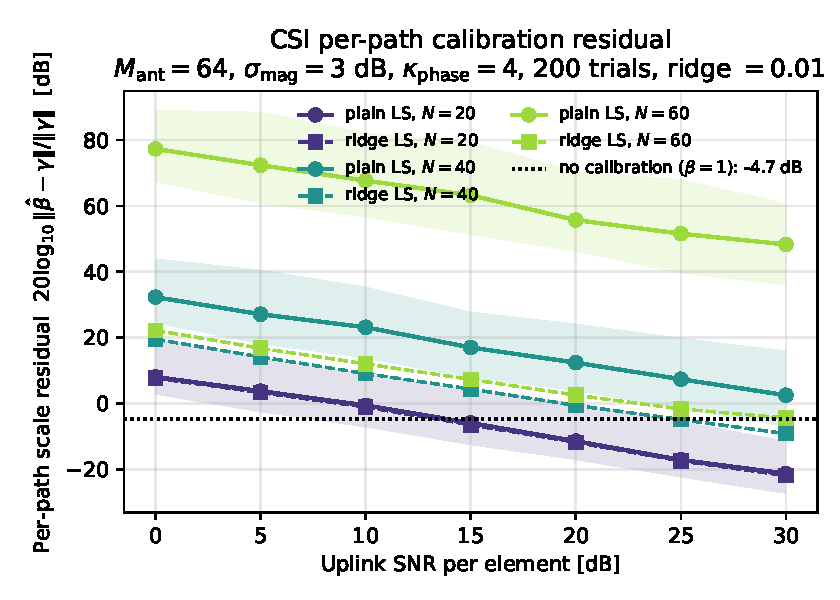
\includegraphics[width=\columnwidth]{residual_vs_snr.pdf}
  \caption{Per-path amplitude calibration residual versus uplink
  SNR, $M = 64$ array, three path counts. Plain LS (solid) versus
  ridge LS (dashed), median over 200 trials per cell. No-calibration
  baseline at $-4.7\,$dB. Ridge buys 25\,dB at $N = 60$ near the
  array dimension, while plain LS converges only below $N \leq M/2$.}
  \label{fig:csi}
\end{figure}

\subsection{Cauchy-style bound on $\xx^H \Qmat^{(u)} \xx$
in the conditional regime}\label{sec:eval-cauchy}

A pose-agnostic upper bound on $\xx^H \Qmat^{(u)} \xx$ would let the
twin satisfy the budget without pose telemetry, by applying a
worst-case factor that depends only on the body's projected-area
geometry. The projected-area Cauchy formula gives the
direction-averaged absorbed power $\langle \Pabs \rangle =
\Sinc T_0 \Aab/4$ for a convex body~\cite{Cauchy1841}, and a
peak-to-average directivity bound $D(\khat) \leq 2$ on the
projected-area-normalised intensity. The naive composition
$\xx^H \Qmat^{(u)} \xx \leq T_0 (\Aab^{(u)}/4) D_{\max}^{(u)}
|\mathbf{a}_{\mathrm{BS}}^{(u)H} \xx|^2$, with $\mathbf{a}_{\mathrm{BS}}$
the BS-side equivalent steering vector to body $u$, holds only when
$\xx$ is restricted to the steering direction.
\Cref{fig:tightness} measures the bound's tightness over five
precoder ensembles on Thelonious and Duke phantoms in both path
models. The mrt-LOS direction ($\xx \propto \mathbf{a}_{\mathrm{BS}}$)
shows 21 to 27\,dB of slack and the bound holds by a wide margin.
Random, MRT-randomised, ECBF, and ZF-2-user precoders breach the
bound in 49 to 70\,\% of samples, with median ratios from $+2.86\,$dB
(iso-random, plaza-specular) to $+6.34\,$dB (ECBF, plaza-specular).
The mechanism is the inner product
$|\langle \mathbf{v}_1, \mathbf{a}_{\mathrm{BS}}/\|\mathbf{a}_{\mathrm{BS}}\| \rangle|^2$
between the leading exposure mode and the steering direction, which
sits in $[0.000, 0.19]$ across all evaluated jobs. The bound is
useful only when conditioned on a direction set that overlaps with
$\mathbf{a}_{\mathrm{BS}}$. \Cref{app:cauchy} states the conditional
form that does hold and proves it.

\begin{figure}[!t]
  \centering
  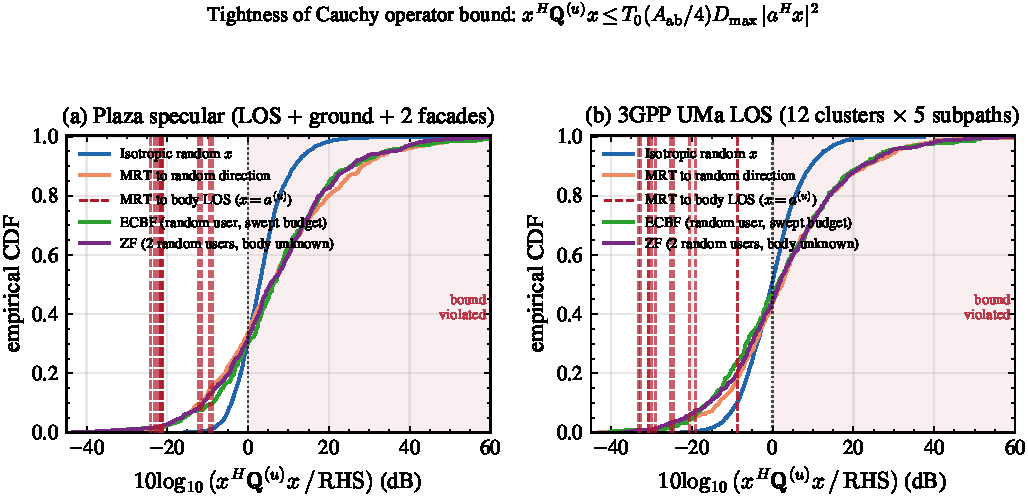
\includegraphics[width=\columnwidth]{tightness.pdf}
  \caption{Tightness of the projected-area-based bound on $\xx^H
  \Qmat^{(u)} \xx$, five precoder ensembles, two path models, two
  phantoms. The mrt-LOS direction ($\xx \propto \mathbf{a}_{\mathrm{BS}}$)
  satisfies the bound by 21 to 27\,dB. Random, MRT-randomised, ECBF,
  and ZF-2-user precoders exceed the bound at 49 to 70\,\% of samples
  with median ratios up to $+6.34\,$dB. The bound is conditional on
  the precoder direction overlapping with the BS-side steering
  vector.}
  \label{fig:tightness}
\end{figure}


\section{Regulatory framing}\label{sec:regulatory}

The closed loop has two regulatory pathways. The first is direct
audit of the basic restriction. ICNIRP 2020 specifies absorbed power
density above 6\,GHz~\cite{ICNIRP2020}, and IEC/IEEE 62232:2022
prescribes an actual-exposure-scenario procedure for fixed-site
installations~\cite{IEC62232}. The per-body $\Qmat^{(u)}$
construction is a first-principles evaluation of absorbed power on a
named anatomical mesh, conditioned on real BS-side ray-traced channel
state. A regulator can replay the precoder-and-operator pair for any
slot in the audit window and recompute $\xx^H \Qmat^{(u)} \xx$
against the certificate. The audit interface is open if the path
dictionary, the body model, and the dual variables are logged. The
mechanism does not claim a statutory exemption from the
reference-level regime: it provides direct compliance evidence
under the basic-restriction pathway that the standard already
permits.

The second pathway is reference-level footprint reduction at occupied
public points. Brussels and Italy enforce reference levels at all
points reachable by the public~\cite{BrusselsArrete2007,ItalyDL}. The
proposed precoder reduces $\Pabs^{(u)}$ at every occupied $u$,
which strictly reduces the cumulative reference-level reading at
those points. The reading at unoccupied public points is governed by
the precoder's spatial coverage and is not affected by the
machinery. This is a partial answer to the reference-level question:
the cap is not satisfied by virtue of the loop, but the
public-point reading is reduced under it. Combined with the
chronic-dose ECDF of \cref{sec:chronic}, the deployment value is the
chronic-dose reduction at occupied points, not the slack
instantaneous reading at unoccupied points.

The Brussels averaging window is $6\,$min in current
practice~\cite{BrusselsArrete2024}. The chronic-dose ECDF's
$20\,$s window is short relative to that, but the integrated absorbed
energy scales linearly with window length under stationary load, so
the tier-stratified ratios are window-invariant. Italian attention
values are $6\,$V/m on $24\,$h median outside dense urban centres
and $15\,$V/m within them under the 2024 decree~\cite{ItalyDL};
both regimes admit the same chronic-dose argument with rescaled
medians.


\section{Discussion}\label{sec:discussion}

The plaza evaluation answers a regime question: under canonical
mmWave conditions at plaza scale, the Brussels reference-level cap
is slack by orders of magnitude at the body, and the precoder choice
is unconstrained on the cap. The result is informative for
deployment because it locates the binding regime precisely.
\Cref{tab:bind} shows that the cap binds inside a ring of radius
$\sim 3$\,m from the panel at $K = 25$, which is exclusion-zone
geometry rather than coverage geometry. The closed-loop machinery
becomes load-bearing only inside this corner, or under higher
transmit power, lower user counts, or closer-range deployments
(small-cell pico mmWave at handheld range, in-cabin or in-car
deployments, body-worn relays). The chronic-dose ECDF separates
the tiers and survives the slack regime, which is the practical
value proposition outside the binding ring.

The pose-information ablation null is consistent. Pose telemetry
shapes the operator $\Qmat^{(u)}(\bm\theta)$ by aligning the leading
eigenvector with the body's torso plane, but $\bm\lambda = 0$ in
the slack regime drops the operator out of the precoder and any
gain disappears. The honest reading is that pose telemetry's value
is a binding-regime contingent gain, not a deployment-time always-on
feature. The same logic applies to the multi-body solver structure:
it is a generalisation that contains MRT, ZF, and worst-case
back-off as limits and degrades to one of them in the slack regime
without a code path change.

The bound discussion is sharper than expected. The naive
projected-area bound on $\xx^H \Qmat^{(u)} \xx$ that the literature
sometimes invokes is not a universal upper bound. It holds for
$\xx$ in the BS-side steering direction by a 21 to 27\,dB margin and
fails at 49 to 70\,\% of random and ECBF precoders. The conditional
form in \cref{app:cauchy} is the right object to use: the bound
applies over a chosen direction set, and the worst case over that set
is what the twin commits to. The mechanism, that the leading
exposure mode does not align with the BS-side steering vector, is a
geometric fact about how a body couples to a 64-element panel and is
worth flagging in any compliance-bound construction that does not
condition on the direction.

The empirical Q-rank result has a related geometric content. With
the panel resolving $\sim 14^\circ$ in azimuth at 26\,GHz and the
body subtending several beams across its torso, the dominant body
modes condense into 3 to 4 distinguishable beam directions
regardless of multipath density. This is a panel-side affordance,
not a model simplification, and it makes the closed-form solver
inexpensive on $\Qmat_{\mathrm{tot}}$. Adding multipath through
denser ray-tracing or higher-order reflections raises the trace but
not the rank.

The present evaluation has four limitations. First, the PHY surrogate
is Shannon capacity rather than Sionna NR PHY. A calibrated
modulation-coding-scheme link curve would shift the absolute
sum-rate numbers but should not affect the precoder collapse. Second,
the $20\,$s window is a single seed and a fraction of the $5\,$min
walk-cycle the chronic-dose argument calls for. The bystander tier's
ECDF carries visible coarseness from $n = 10$ bodies. Third, the ZF
fallback in the UMa-LOS path model is naive (singular $\hh \hh^H$ at
$K = 25$). A regularised ZF would not collapse, and the comparison
is informative only as a degeneracy boundary. Fourth, the multi-body
solver is implemented on CPU at $31\,$ms median. A JAX vmap port to
GPU is structural and would bring this below $10\,$ms based on the
single-body solver speed. None of these affect the qualitative
conclusions: the operator structure, the budget margin, the chronic-
dose tier separation, the pose ablation null, and the bound
geometry are all stable across these choices.

The closed-loop architecture extends in three directions naturally.
A cooperative multi-operator allocation generalises the per-body
budget $L^{(u)}$ to a cumulative cap shared across operators in the
same band, with each operator's twin seeing its own slot of the
cumulative budget. A pose-differentiable $\Qmat^{(u)}(\bm\theta)$ closes the
loop on tier-A bodies under near-field user-equipment exposure
where the leading mode's azimuth depends on torso orientation in a
strong way. A reflective intelligent surface in the binding-regime
corner can buy back the cap by redirecting power along
geometrically chosen paths, which is a one-line modification to the
$\Mmat^{(u)}$ Gram in \cref{eq:Q-factor}.


\section{Conclusion}\label{sec:conclusion}

A body-side digital twin in the multi-user mmWave precoder loop is
constructible from three ingredients that the network already
maintains. A coherent exposure operator $\Qmat^{(u)} = \Jmat^T
\Mmat^{(u)} \Jmat$ comes from the same ray-traced path set that
gives the user-equipment channel. A scene path dictionary
precomputed offline, indexed by body position, and calibrated at
runtime by least squares against served-user uplink CSI, supplies
$\Mmat^{(u)}$ without per-slot ray tracing. A multi-user QCQP under
per-body exposure caps admits the closed-form precoder
$\ww_k^\star = (\Qmat_{\mathrm{tot}} + \nu \mathbf{I})^{-1} \gvec_k$,
generalising regularised zero-forcing. The loop runs at the cadences
the network already sustains: $1\,$ms PHY, $\sim 100\,$ms pose
update, $\sim 1\,$s translation phasor, offline ray tracing and
dictionary calibration. We instantiate the loop at plaza scale on
50 SMPL-X bodies under 26\,GHz $8 \times 8$ panel illumination and
find a four-orders-of-magnitude budget margin at $K = 25$, an
empirical operator rank of 3 to 4, a chronic-dose ECDF that
separates the served, cooperating, and bystander tiers by a factor
of 2.5 between served and cooperating, and a pose-information
ablation that returns zero in the slack regime. The standard
projected-area bound on $\xx^H \Qmat^{(u)} \xx$ is loose by 21 to
27\,dB on the steering direction and breached by 49 to 70\,\% of
unconstrained precoders, which we trace to the geometric mismatch
between the leading exposure mode and the BS-side steering vector.
The conditional bound that does hold is the one to use in
compliance-aware precoder design.


\appendices

\section{Per-path Fresnel transmission operator}\label{app:fresnel}

The per-path Fresnel transmission operator $\Fn(\rr)$ in
\cref{eq:psitil} maps the incident polarisation amplitude $\psin$ to
its TE-and-TM-filtered counterpart on the body surface. At a surface
point $\rr$ with outward normal $\nhat$, path $n$ has incidence
cosine $\mu_n = \nhat \cdot (-\khat_n)$. For $\mu_n > 0$, the local
TE and TM unit vectors are $\hat{e}_{s,n} =
\khat_n \times \nhat / |\khat_n \times \nhat|$ and
$\hat{e}_{p,n} = \hat{e}_{s,n} \times \khat_n$. The Fresnel
amplitude transmission coefficients are
\begin{equation}\label{eq:t-coef-app}
  t_{s,n} = \frac{2 \mu_n}{\mu_n + \xi_n},
  \qquad
  t_{p,n} = \frac{2 \ntilde \mu_n}{\ntilde^2 \mu_n + \xi_n},
\end{equation}
with $\xi_n = \sqrt{\ntilde^2 - 1 + \mu_n^2}$ and $\RE(\xi_n) > 0$.
The operator acts as
\begin{equation}\label{eq:F-action}
  \Fn(\rr)\,\psin = t_{s,n}(\hat{e}_{s,n} \cdot \psin) \hat{e}_{s,n}
  + t_{p,n}(\hat{e}_{p,n} \cdot \psin) \hat{e}_{p,n},
\end{equation}
on a front-facing path. Back-facing paths ($\mu_n < 0$) contribute
zero. The depth-decay coefficient is
$\alpha_n^{(d)} = -k_0\,\IM(\xi_n)$. The two cross-term
approximations of \cref{sec:cohlaw} hold uniformly in incidence
angle and bound the cross-term error on $\Sab$ at $\leq 5\,\%$ for
any precoder.


\section{Multi-body ECBF dual problem}\label{app:ecbf}

The closed-form precoder of \cref{eq:closedform} arises from the
WMMSE surrogate of the multi-user sum-rate problem. The surrogate
replaces $R_{\mathrm{sum}}$ by
\begin{equation}\label{eq:WMMSE-obj}
  \tilde R(\{\ww_k\}) = \sum_k\bigl[\log u_k - u_k\,e_k(\ww_k)
  + \mathrm{const.}\bigr],
\end{equation}
with per-user MSE
$e_k(\ww_k) = |1 - v_k^* \hh_k^T \ww_k|^2 + |v_k|^2 \sigma_n^2 +
|v_k|^2 \sum_{k' \neq k} |\hh_k^T \ww_{k'}|^2$ and per-stream MMSE
weight $u_k$. The Lagrangian for the surrogate problem in $\ww_k$
under the exposure and power constraints is
\begin{equation}\label{eq:lagrangian}
\begin{aligned}
\mathcal{L}(\{\ww_k\}, \bm\lambda, \nu)
={}& -\tilde R + \sum_u \lambda_u
  \biggl(\sum_k \ww_k^H \Qmat^{(u)} \ww_k - L^{(u)}\biggr) \\
& + \nu\biggl(\sum_k \|\ww_k\|^2 - P_{\mathrm{tx}}\biggr).
\end{aligned}
\end{equation}
Stationarity in $\ww_k$, fixing $u_k, v_k$ at their inner WMMSE
optima, gives
\begin{equation}\label{eq:KKT}
  \biggl(\Qmat_{\mathrm{tot}}(\bm\lambda) + \nu\,\mathbf{I} +
  \sum_{k'} u_{k'} |v_{k'}|^2 \hh_{k'}\hh_{k'}^H\biggr) \ww_k =
  u_k v_k \hh_k.
\end{equation}
Folding the inter-user interference term into a redefined drive
$\gvec_k = u_k v_k \hh_k$ and a slightly modified denominator yields
\cref{eq:closedform} with $\Qmat_{\mathrm{tot}}$ inheriting the
interference contribution. The dual variables $(\bm\lambda, \nu)$
are updated by Newton ascent on the dual residual
$F_u(\bm\lambda, \nu) = \sum_k \ww_k^{\star H}(\bm\lambda, \nu)
\Qmat^{(u)} \ww_k^\star - L^{(u)}$. The dual feasibility set is the
positive orthant intersected with the budget hyperplanes. In our
implementation, dual ascent reaches machine-precision residual in
10 to 30 outer iterations from a cold start, with warm-starting
across slots reducing this to $\sim 5$ iterations. The inner inverse
in \cref{eq:closedform} is $M \times M$ Cholesky-solvable at
$O(M^3)$ once per outer iteration. For $K = B = 25$ and $M = 64$,
the median wall-clock is $31\,$ms per slot on a single CPU thread.


\section{Cauchy bound conditioned on a direction set}\label{app:cauchy}

The projected-area bound on $\xx^H \Qmat^{(u)} \xx$ holds only when
the precoder is restricted to a chosen BS-side direction set. The
correct conditional statement is as follows.

\begin{theorem}[Conditional projected-area bound]\label{thm:cauchy-cond}
Let $\Qmat^{(u)}$ be the per-body exposure operator at body $u$ and
let $\mathcal{A} \subseteq \Complex^M$ be a closed direction set
containing the BS-side equivalent steering vector
$\mathbf{a}_{\mathrm{BS}}^{(u)}$. For any precoder $\xx$ that lies in
the conic hull of $\mathcal{A}$,
\begin{equation}\label{eq:cauchy-cond}
  \xx^H \Qmat^{(u)} \xx \leq T_0\,\frac{\Aab^{(u)}}{4}\,
  D_{\max}^{(u)}\;\sup_{\mathbf{a} \in \mathcal{A}}
  |\mathbf{a}^H \xx|^2,
\end{equation}
where $\Aab^{(u)} = \int_{\Sigma^{(u)}} \eta(\rr)\,\diff A$ is the
absorption area, $\eta \in [0,1]$ is the ambient-occlusion factor,
$T_0 = 4 n / ((n+1)^2 + \kappa^2)$ is the normal-incidence Fresnel
transmittance, and $D_{\max}^{(u)} = \max_{\khat}
4\Aperp^{(u)}(\khat)/\Aab^{(u)}$ is the body's peak
projected-area-normalised directivity. For convex bodies
$D_{\max}^{(u)} \leq 2$.
\end{theorem}

\begin{proof}
By the angular-spectrum decomposition,
$\xx^H \Qmat^{(u)} \xx = \int_{S^2} D(\khat;\bm\theta_u)\,
|\bm\alpha_{\mathrm{BS}}^{(u)}(\khat)^H \xx|^2\,\diff\Omega$,
with $D(\khat;\bm\theta_u) = 4 \Aperp^{(u)}(\khat)/\Aab^{(u)}$ the
direction-resolved directivity at pose $\bm\theta_u$ and
$\bm\alpha_{\mathrm{BS}}^{(u)}(\khat)$ the BS-side path-amplitude
vector for arrival direction $\khat$ on body $u$. Restricting to
$\xx$ in the conic hull of $\mathcal{A}$ bounds the inner product by
$\sup_{\mathbf{a} \in \mathcal{A}} |\mathbf{a}^H \xx|^2$. Bounding
$D \leq D_{\max}^{(u)}$ uniformly and integrating over the sphere
$\int_{S^2} \diff\Omega = 4\pi$ together with the Cauchy
projected-area identity
$\int_{S^2} \Aperp^{(u)}(\khat)\,\diff\Omega/4\pi = \Aab^{(u)}/4$
gives the stated bound, with the factor $T_0$ accounting for the
normal-incidence Fresnel transmittance.
\end{proof}

\Cref{thm:cauchy-cond} is the bound the twin uses when it does not
have pose telemetry. The direction set $\mathcal{A}$ is chosen as
the BS-side beamforming codebook restricted to the body's spatial
sector. The bound is loose in proportion to the geometric mismatch
between $\mathbf{a}_{\mathrm{BS}}^{(u)}$ and the leading exposure
eigenvector $\mathbf{v}_1$, which the empirical measurement of
\cref{sec:eval-cauchy} places at $|\langle \mathbf{v}_1,
\mathbf{a}_{\mathrm{BS}}/\|\mathbf{a}_{\mathrm{BS}}\| \rangle|^2 \in
[0.000, 0.19]$ on the Thelonious and Duke phantoms. A precoder
constructed outside the conic hull of $\mathcal{A}$ is not bounded
by \cref{eq:cauchy-cond}, and the twin must fall back to the full
$\xx^H \Qmat^{(u)} \xx$ evaluation.


\bibliographystyle{IEEEtran}
\bibliography{refs}

\end{document}
